% Foliensatz: "AFu-Kurs nach DJ4UF" von DK0TU, Amateurfunkgruppe der TU Berlin
% Lizenz: CC BY-NC-SA 3.0 de (http://creativecommons.org/licenses/by-nc-sa/3.0/de/)
% Autoren: Sebastian Lange <dl7bst@dk0tu.de>
% Korrekturen: Lars Weiler <dc4lw@darc.de>

\documentclass[aspectratio=169]{beamer}

\usepackage[ngerman]{babel} % deutsche Worttrennung etc.
\usepackage[utf8]{inputenc} % UTF8 Text

\usepackage[super, comma, numbers, square, sort]{natbib}

\usepackage{hyperref}       % Hyperref Package für bessere Referenzen (todo)
\hypersetup{
	colorlinks=false,       %   false: boxed links; true: colored links
    %linkcolor=white,       %   color of internal links (change box color with linkbordercolor)
    citecolor=red,          %   color of links to bibliography
    filecolor=white,        %   color of file links
    urlcolor=blue           %   color of external links
}

\usepackage{multirow}
\usepackage{wasysym}  % Math Symbols like \permil
%\usepackage{colortbl}
%\usepackage{subscript}
%\usepackage{caption}
%\usepackage{setspace}
%\usepackage{xcolor}        % benutze CodeListe

% Footnote
%\usepackage{hanging}
%
%\setbeamertemplate{footnote}{%
%  \hangpara{2em}{1}%
%  \makebox[2em][l]{\insertfootnotemark}\footnotesize\insertfootnotetext\par%
%}


%\usepackage{pgf}
%\usepackage{tikz}
%\usetikzlibrary{arrows,automata}
%\usetikzlibrary{positioning}
%
%\tikzset{
%    state/.style={
%           rectangle,
%           rounded corners,
%           draw=black, very thick,
%           minimum height=2em,
%           minimum width=2pt,
%           inner sep=2pt,
%           text centered,
%           },
%}

%\usepackage{listings}
%\lstset{basicstyle=\small, numberstyle=\tiny, extendedchars=true, numbers=left, numbersep=5pt}
%\lstset{showtabs=false, showspaces=false, showstringspaces=false}
%%\lstset{backgroundcolor=\color{white!75!lightgray}, , frame=single}
%%\lstset{backgroundcolor=\color{white}}
%%\lstset{backgroundcolor=none}
%\lstset{keywordstyle=\color{blue!50!gray},  identifierstyle=\color{black}}
%\lstset{commentstyle=\color{green!50!gray}, stringstyle=\color{red!50!gray}}
%\lstset{language=C, fontadjust=true, tabsize=2, breaklines=true}
%\lstset{backgroundcolor=\color{white!75!lightgray}, caption=\lstname, frame=single}
%\lstset{emphstyle=\color{black}\fbox}
%
%% Keine "Listing:"-Caption
%\captionsetup{labelformat=empty,labelsep=none}
%
%% für mathematische Umgebungen
%\usepackage{amsmath,amsfonts,amssymb}
%
%\lstdefinestyle{Bash}{
%language=Bash,
%frame=single,
%rulecolor=\color{black},
%backgroundcolor=\color{gray!50},
%keywordstyle=\color{black},
%identifierstyle=,
%commentstyle=\color{black},
%stringstyle=\color{magenta!65!white},
%showstringspaces=false,
%basicstyle=\footnotesize\ttfamily\color{black},
%numbers=none,
%breaklines=true,
%captionpos=b
%}

%\usepackage{listings}
%
%\lstdefinestyle{basic}{
%    captionpos=t,%
%    basicstyle=\footnotesize\ttfamily,%
%    numberstyle=\tiny,%
%    numbers=left,%
%    stepnumber=1,%
%    frame=single,%
%    showspaces=false,%
%    showstringspaces=false,%
%    showtabs=false,%
%    %
%    keywordstyle=\color{blue},%
%    identifierstyle=,%
%    commentstyle=\color{gray},%
%    stringstyle=\color{magenta}%
%}



% fließende Boxen haben keinen Abstand
%\fboxsep0mm

% inkludiere Creative Commons Helper
%%%%%%%%%%%%%%%%%%%%%%%%%%%%%%%%%%%%%%%%%%%%%%%%%%%%%%%%%%%%%%%%
%% ccBeamer 0.1, 2007-07-02                                   %%
%% Written by Sebastian Pipping <webmaster@hartwork.org>      %%
%% ---------------------------------------------------------- %%
%% Licensed under Creative Commons Attribution-ShareAlike 3.0 %%
%% http://creativecommons.org/licenses/by-sa/3.0/             %%
%%%%%%%%%%%%%%%%%%%%%%%%%%%%%%%%%%%%%%%%%%%%%%%%%%%%%%%%%%%%%%%%


%% Images
\newcommand{\CcImageBy}[1]{%
	
\includegraphics[scale=#1]{texdata/creative_commons/cc_by_30.pdf}%
}
\newcommand{\CcImageCc}[1]{%
	
\includegraphics[scale=#1]{texdata/creative_commons/cc_cc_30.pdf}%
}
\newcommand{\CcImageDevNations}[1]{%
	
\includegraphics[scale=#1]{texdata/creative_commons/cc_dev_nations_30.pdf}%
}
\newcommand{\CcImageNc}[1]{%
	
\includegraphics[scale=#1]{texdata/creative_commons/cc_nc_30.pdf}%
}
\newcommand{\CcImageNd}[1]{%
	
\includegraphics[scale=#1]{texdata/creative_commons/cc_nd_30.pdf}%
}
\newcommand{\CcImagePd}[1]{%
	
\includegraphics[scale=#1]{texdata/creative_commons/cc_pd_30.pdf}%
}
\newcommand{\CcImageSa}[1]{%
	
\includegraphics[scale=#1]{texdata/creative_commons/cc_sa_30.pdf}%
}
\newcommand{\CcImageSampling}[1]{%
	
\includegraphics[scale=#1]{texdata/creative_commons/cc_sampling_30.pdf}%
}
\newcommand{\CcImageSamplingPlus}[1]{%
	
\includegraphics[scale=#1]{texdata/creative_commons/cc_sampling_plus_30.pdf}%
}


%% Groups
\newcommand{\CcGroupBy}[2]{% zoom, gap
	\CcImageCc{#1}\hspace*{#2}\CcImageBy{#1}%
}
\newcommand{\CcGroupByNc}[2]{% zoom, gap
	\CcImageCc{#1}\hspace*{#2}\CcImageBy{#1}\hspace*{#2}\CcImageNc{#1}%
}
\newcommand{\CcGroupByNcNd}[2]{% zoom, gap
	\CcImageCc{#1}\hspace*{#2}\CcImageBy{#1}\hspace*{#2}\CcImageNc{#1}\hspace*{#2}\CcImageNd{#1}%
}
\newcommand{\CcGroupByNcSa}[2]{% zoom, gap
	\CcImageCc{#1}\hspace*{#2}\CcImageBy{#1}\hspace*{#2}\CcImageNc{#1}\hspace*{#2}\CcImageSa{#1}%
}
\newcommand{\CcGroupByNd}[2]{% zoom, gap
	\CcImageCc{#1}\hspace*{#2}\CcImageBy{#1}\hspace*{#2}\CcImageNd{#1}%
}
\newcommand{\CcGroupBySa}[2]{% zoom, gap
	\CcImageCc{#1}\hspace*{#2}\CcImageBy{#1}\hspace*{#2}\CcImageSa{#1}%
}
\newcommand{\CcGroupDevNations}[2]{% zoom, gap
	\CcImageCc{#1}\hspace*{#2}\CcImageDevNations{#1}%
}
\newcommand{\CcGroupNcSampling}[2]{% zoom, gap
	\CcImageCc{#1}\hspace*{#2}\CcImageNc{#1}\hspace*{#2}\CcImageSampling{#1}%
}
\newcommand{\CcGroupPd}[1]{% zoom
	\CcImagePd{#1}%
}
\newcommand{\CcGroupSampling}[1]{% zoom
	\CcImageSampling{#1}%
}
\newcommand{\CcGroupSamplingPlus}[1]{% zoom
	\CcImageSamplingPlus{#1}%
}


%% Text
\newcommand{\CcLongnameBy}{Attribution}
\newcommand{\CcLongnameByNc}{Attribution-NonCommercial}
\newcommand{\CcLongnameByNcNd}{Attribution-NoDerivs}
\newcommand{\CcLongnameByNcSa}{Attribution-NonCommercial-ShareAlike}
\newcommand{\CcLongnameByNd}{Attribution-NoDerivs}
\newcommand{\CcLongnameBySa}{Attribution-ShareAlike}

\newcommand{\CcNote}[1]{% longname
	This work is licensed under the \textit{Creative Commons #1 3.0 License}.%
}


% generelles Thema auswählen
\usetheme{Goettingen} %Berlin spart ohne Sidebar allerdings angenehm Platz
% AnnArbor | Antibes | Bergen | Berkeley | Berlin | Boadilla | boxes | CambridgeUS | Copenhagen | Darmstadt | default | Dresden | Frankfurt | Goettingen | Hannover | Ilmenau | JuanLesPins | Luebeck | Madrid | Malmoe | Marburg | Montpellier | PaloAlto | Pittsburgh | Rochester | Singapore | Szeged | Warsaw

% Farben wählen
\usecolortheme{beetle}
% beaver | beetle | crane | default | dolphin | dove | fly | lily | orchid | rose | seagull | seahorse | sidebartab | structure | whale | wolverine

% Setze alle Farben auf Grau und Weiß
%\definecolor{craneorange}{RGB}{64,64,64}
%\definecolor{craneblue}{RGB}{255,255,255}

% Schriftart wählen
\usefonttheme{default}
% default | professionalfonts | serif | structurebold | structureitalicserif | structuresmallcapsserif

% Innere Themen(Kopf-, Fuß-, Sidebar usw)
%\useinnertheme{default}
\useinnertheme{circles}
% default | inmargin | rectangles | rounded | circles

% Äußere Themen (Anordnung der inneren, grenzen der Folien etc.)
\useoutertheme{infolines}
% default | infolines | miniframes | shadow | sidebar | smoothbars | smoothtree | split | tree

% Deaktiviere Navigations-Symbole ({} -> leer)
\setbeamertemplate{navigation symbols}{}
%\setbeamertemplate{navigation symbols}{\large \ifnum \insertframenumber <10 0\fi\insertframenumber/\inserttotalframenumber\vspace*{0.2ex}}

% Zeige ein Hintergrundbild
\setbeamertemplate{background canvas}{
        \hspace*{-2.0cm}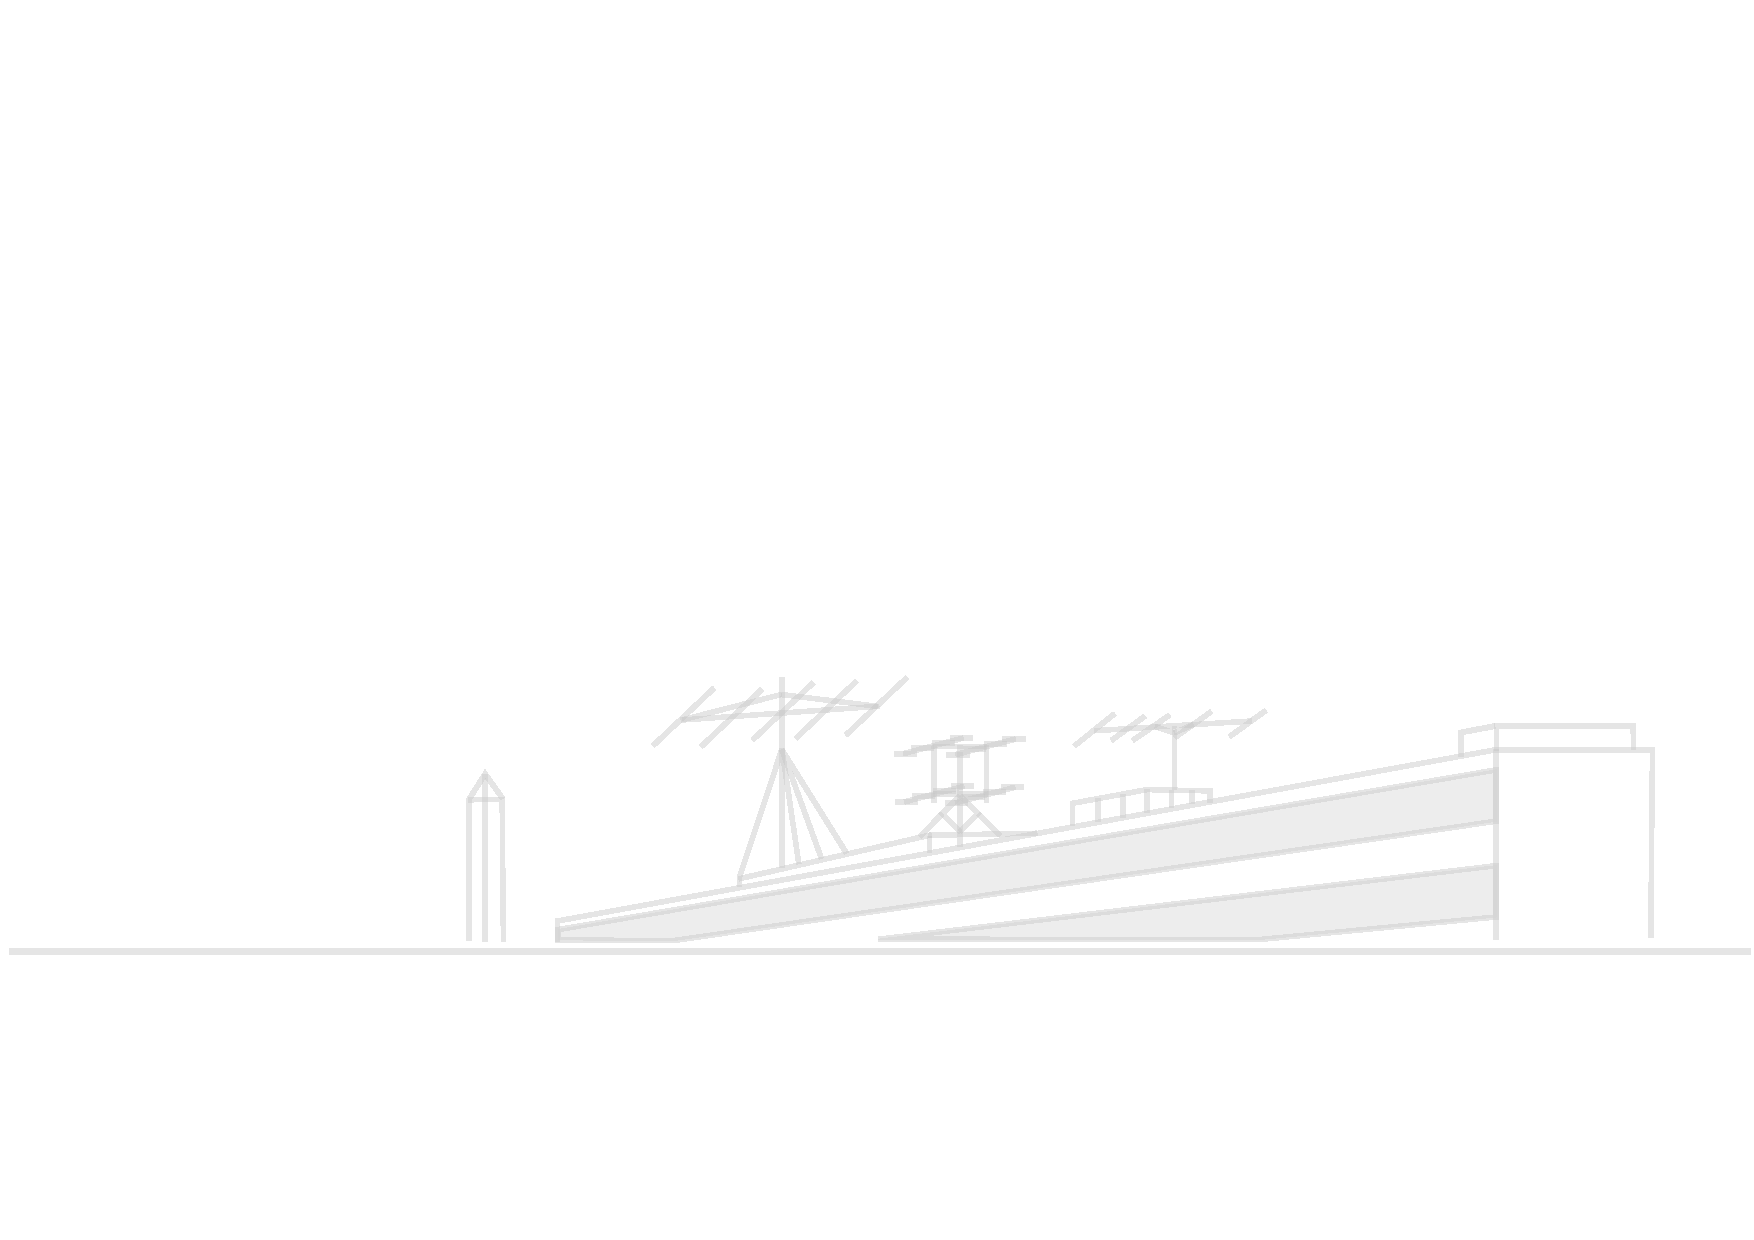
\includegraphics[width=17.8cm]{texdata/dk0tu_rooftop_background.pdf}
}

% Foliennummer einfügen
\setbeamertemplate{footline}[frame number]
%\setbeamertemplate{footline}{}

% Ändere das Zeichen vor jedem item
%\setbeamertemplate{itemize item}{\color{craneorange}$\blacktriangleright$}
%\setbeamertemplate{itemize subitem}{\color{craneorange}$\triangleright$}
%\setbeamertemplate{itemize subsubitem}{\color{craneorange}$\blacktriangleright$}

% Ändert die Blöcke 
\setbeamertemplate{blocks}[rounded][shadow=true]
% default | rounded [shadow=true|false]

%
% Eigene Kommandos
%

% Hack to get natbib and beamer working together. "The beamer user guide suggests
% that only the manual bibliography entry approach is supported"
% on some system it works out of the box, sometimes you need the hack :-(
% so check it --dl7bst
\ifdefined\newblock
    \relax
\else
    \newcommand{\newblock}{}
\fi

% \includedia command to generate png out of a dia file
% NEEDS installed dia and pdflatex option --shell-escape
\newcommand{\includedia}[1]{
    \immediate\write18{/usr/bin/dia #1.dia -e #1_diatmp.png -t png}
}

% RICHIG GROSSER FONT!
\newfont{\bigfont}{cmr10 at 144pt}
\newfont{\smallfont}{cmr10 at 8pt}

% Römische Ziffern
\makeatletter
\newcommand{\rmnum}[1]{\romannumeral #1}
\newcommand{\Rmnum}[1]{\expandafter\@slowromancap\romannumeral #1@}
\makeatother

% Schwarze Überschrift
%\setbeamercolor{frametitle}{fg=black}
%\setbeamercolor{title}{fg=black}

% Item- und Box-Farben
\definecolor{deepBlue}{HTML}{000066}
\setbeamercolor{itemize item}{fg=deepBlue}
\setbeamercolor{itemize subitem}{fg=deepBlue}
\setbeamercolor{description item}{fg=deepBlue}
\setbeamercolor{block title}{fg=deepBlue!100, bg=blue!15}
\setbeamercolor{block body}{fg=black, bg=blue!5}
\setbeamercolor{block title alerted}{fg=deepBlue, bg=red!75}
\setbeamercolor{block body alerted}{fg=black, bg=red!15}
\setbeamercolor*{block title example}{fg=blue!50, bg=blue!10}
\setbeamercolor*{block body example}{fg= blue, bg=blue!5}

%\setbeamercolor{section in head/foot}{parent=palette primary}
%\setbeamercolor{subsection in head/foot}{parent=palette secondary}
%\setbeamercolor{sidebar}{fg=darkblue,bg=yellow!90!orange}
%\setbeamercolor{title in sidebar}{fg=darkblue}
%\setbeamercolor{author in sidebar}{fg=darkblue}
%\setbeamercolor{section in sidebar}{fg=darkblue!10!black}
%\setbeamercolor{subsection in sidebar}{fg=darkblue!50!black}

% Titlepage Infos
\title{AFu-Kurs nach DJ4UF}
\author[DKØTU]{DKØTU\\ \footnotesize{Amateurfunkgruppe der TU Berlin}}
\institute[DKØTU]{\url{http://www.dk0tu.de} }

% PDF-Eigenschaften
\subject{DK0TU-Amateurfunkkurs nach DJ4UF}
\keywords{Amateurfunk Kurs HAM Radio Course CC-BY-NC-SA OpenSource TU Berlin DK0TU}

\subtitle{Betriebstechnik/Vorschriften 02:         \\
  Das ``Internationale Buchstabieralphabet'' \\[2em]}
\date{Stand 10.10.2016}
 \begin{document}

\begin{frame}
    \titlepage
    \vfill
    \begin{center}
        \ccbyncsaeu\\
        {\tiny This work is licensed under the \em{Creative Commons Attribution-NonCommercial-ShareAlike 3.0 License}.}\\[0.5ex]
         \tiny Amateurfunkgruppe der Technische Universität Berlin (AfuTUB), DKØTU
         %\includegraphics[scale=0.5]{img/DK0TU_Logo.pdf}
    \end{center}
\end{frame}


\section*{Einleitung}

\begin{frame}
  \frametitle{Einleitung / Buchstabieralphabete}
  \begin{center}
    \Large{Wozu braucht man das?} \\
    \Large{Welche kennt ihr?}
  \end{center}
\end{frame}

\begin{frame}
  \frametitle{Einleitung / Buchstabieralphabete}

  Vermeidung von Verwechslungen (bei englischer Aussprache):

  \begin{itemize}
    \item D vs. G vs. T vs. E
    \item J vs. A
    \item Q vs. U
    \item Y vs. I
    \item je nach Dialekt und Aussprache einige mehr
  \end{itemize}

  Viele verschiende nationale und internationale Buchstabieralphabete. Wir
  verwenden nicht das deutsche.

\end{frame}

\section*{Buch\-stabier\-tafel}

\begin{frame}
  \frametitle{Buchstabiertafel / Zusammentragen}

  Laut Radio Regulations (RR) verwenden wir das internationale Alphabet
  (ITU\footnote{\tiny International Telecommunication
  Union}/ICAO\footnote{\tiny International Civil Aviation
  Organization}/NATO\footnote{\tiny North Atlantic Treaty Organization}).

  Nicht nur für die Prüfung wichtig, sondern für die Praxis. Die Benutzung
  trainiert.

  \begin{exampleblock}{Buchstabierwörter}
    Aufgabe: Gemeinsames Zusammentragen der Buchstabierwörter!
  \end{exampleblock}

  Audio Check: \emph{NATO Phonetic Alphabet reading}
  \footnote{\tiny \url{http://commons.wikimedia.org/wiki/File:NATO_Phonetic_Alphabet_reading.ogg}}

\end{frame}

\begin{frame}
  \frametitle{Buchstabiertafel / gesamte Tabelle}

  \begin{center}
    \scriptsize
    \begin{tabular}{|l|l|||l|l|}\hline
      Zeichen           & Phonetik      & Zeichen          & Phonetik       \\ \hline \hline
      \textbf{A}lfa     & (AL-FAH)      & \textbf{S}ierra  & (SEE-AIR-RAH)  \\ \hline
      \textbf{B}ravo    & (BRAH-VOH)    & \textbf{T}ango   & (TANG-GO)      \\ \hline
      \textbf{C}harlie  & (SHAR-LEE)    & \textbf{U}niform & (YOU-NEE-FORM) \\ \hline
      \textbf{D}elta    & (DELL-TAH)    & \textbf{V}ictor  & (VIK-TAH)      \\ \hline
      \textbf{E}cho     & (ECK-OH)      & \textbf{W}hiskey & (WISS-KEY)     \\ \hline
      \textbf{F}oxtrot  & (FOKS-TROT)   & \textbf{X}ray    & (ECKS-RAY)     \\ \hline
      \textbf{G}olf     & (GOLF)        & \textbf{Y}ankee  & (YANG-KEY)     \\ \hline
      \textbf{H}otel    & (HOH-TEL)     & \textbf{Z}ulu    & (ZOO-LOO)      \\ \hline
      \textbf{I}ndia    & (IN-DEE-AH)   & \textbf{0} Zero  & (ZEE-RO)       \\ \hline
      \textbf{J}uliett  & (JEW-LEE-ETT) & \textbf{1} One   & (WUN)          \\ \hline
      \textbf{K}ilo     & (KEY-LOH)     & \textbf{2} Two   & (TOO)          \\ \hline
      \textbf{L}ima     & (LEE-MAH)     & \textbf{3} Three & (TREE)         \\ \hline
      \textbf{M}ike     & (MIKE)        & \textbf{4} Four  & (FOW-ER)       \\ \hline
      \textbf{N}ovember & (NO-VEM-BER)  & \textbf{5} Five  & (FIFE)         \\ \hline
      \textbf{O}scar    & (OSS-CAH)     & \textbf{6} Six   & (SIX)          \\ \hline
      \textbf{P}apa     & (PAH-PAH)     & \textbf{7} Seven & (SEV-EN)       \\ \hline
      \textbf{Q}uebec   & (KEH-BECK)    & \textbf{8} Eight & (AIT)          \\ \hline
      \textbf{R}omeo    & (ROW-ME-OH)   & \textbf{9} Nine  & (NIN-ER)       \\ \hline
    \end{tabular}
  \end{center}

\end{frame}


\begin{frame}
  \frametitle{Buchstabiertafel / Anmerkungen}

  Gerade im deutschen Raum Vorsicht mit: \\
  \textbf{Y}ankee (kein J) und \textbf{Z}ulu (kein S). \\[2em]

  Für die \textbf{Praxis} im Hinterkopf behalten: \\
  Verwechslungen können dennoch möglich sein. Es bietet sich an einige
  Alternativen/Ergänzungen zu kennen und ggf. zu verwenden z.B.
  \begin{itemize}
    \item \textbf{H}onolulu
    \item \textbf{I}taly
    \item \textbf{R}adio
    \item \textbf{S}ugar
    \item \textbf{T}okyo
    \item \textbf{U}nited
  \end{itemize}

\end{frame}

\begin{frame}
  \frametitle{Alternativen / Beispiel DKØTU}

  \only<1>{Buchstabiert?}

  \pause

  Oft verstanden als \emph{Delta Kilo Zero \textbf{Echo} Uniform} \\[2em]

  \pause

  Alternativen: \emph{Tokyo/Texas United}
  \footnote{Disclaimer: Nicht von alten/alternativen
  Buchstabieralphabeten verwirren lassen: Romeo, Radio, Russia...!}\\[2em]
  Problematisch kann auch z.B. Y vs. W sein.

\end{frame}


\section*{Übung}

\begin{frame}

  \begin{center}
    \begin{figure}
      
\includegraphics[width=\textwidth,height=.9\textheight,keepaspectratio]{bv02/na_bravo_meme.jpg}
      \attribcaption{Na Bravo}{“Der Postillon”}{http://www.der-postillon.com/2013/02/newsticker-414.html}{}
    \end{figure}
  \end{center}

\end{frame}

\begin{frame}
  \frametitle{Übung: Buchstabieren von Pangrammen\footnote{https://de.wikipedia.org/wiki/Pangramm}}

  \begin{exampleblock}{Aufgabe: Verwendet das internat. Buchstabieralphabet!}

    \only<1>{\uppercase{The quick brown fox jumps over the lazy dog}}

    \only<2>{\uppercase{Franz jagt im komplett verwahrlosten Taxi quer durch Bayern}}

    \only<3>{\uppercase{Falsches Üben von Xylophonmusik quält jeden größeren Zwerg}}

    \only<4>{\uppercase{Prall vom Whisky flog Quax den Jet zu Bruch}}

    \only<5>{\uppercase{The five boxing wizards jump quickly.}}

    \only<6>{\uppercase{MS ``Fliegerkosmonaut der DDR Sigmund
    Jähn''}\footnote{ehem. Frachtschiff der DDR und
    beliebt den Funker zum Buchstabieren aufzufordern}}

    % Vogel Quax zwickt Johnys Pferd Bim
    % Zwölf Boxkämpfer jagen Viktor quer über den großen Sylter Deich

  \end{exampleblock}

\end{frame}

\begin{frame}
  \frametitle{Übung: Buchstabieren und Aufschreiben}

  \begin{alertblock}{Hausaufgabe}
    Das Internationale Buchstabieralphabet nebenbei auswendig lernen:
    Einfach alles möglich sich selbst buchstabieren. Zum Beispiel
    Kfz-Kennzeichen, Werbung in der U-Bahn, etc.
  \end{alertblock}

  \begin{alertblock}{Aufgabe: Buchstabiert euren Namen!}
    Den eigenen Namen komplett buchstabieren können -- beim nächsten Mal
    wird zufällig jemand ausgewählt und alle anderen müssen mitschreiben.
  \end{alertblock}

\end{frame}

\section*{Referenzen}

\begin{frame}
  \frametitle{Referenzen/Links}

  \footnotesize
  \begin{itemize}
    \item Moltrecht B/V 02: \\
      \url{https://www.darc.de/der-club/referate/ajw/lehrgang-bv/bv02/}
    \item Wikipedia DE: \\
      \url{http://de.wikipedia.org/wiki/Buchstabiertafel}
    \item Wikipedia EN: \\
      \url{http://en.wikipedia.org/wiki/NATO_phonetic_alphabet}
  \end{itemize}

\end{frame}

% Hier könnte noch eine Kontaktfolie stehen

\end{document}

